%latex model.tex
%bibtex model
%latex model.tex
%latex model.tex
%pdflatex model.tex

%it's possible to work online (e.g. www.overleaf.com)


\documentclass[runningheads,a4paper,11pt]{report}

\usepackage{algorithmic}
\usepackage{algorithm} 
\usepackage{array}
\usepackage{amsmath}
\usepackage{amsfonts}
\usepackage{amssymb}
\usepackage{amsthm}
\usepackage{caption}
\usepackage{comment} 
\usepackage{epsfig} 
\usepackage{fancyhdr}
\usepackage[T1]{fontenc}
\usepackage{geometry} 
\usepackage{graphicx}
\usepackage[colorlinks]{hyperref} 
\usepackage[latin1]{inputenc}
\usepackage{multicol}
\usepackage{multirow} 
\usepackage{rotating}
\usepackage{setspace}
\usepackage{subfigure}
\usepackage{url}
\usepackage{verbatim}
\usepackage{xcolor}
\usepackage{tikz}
\usetikzlibrary{arrows.meta, positioning, shapes.geometric}

\geometry{a4paper,top=3cm,left=2cm,right=2cm,bottom=3cm}

\pagestyle{fancy}
\fancyhf{}
\fancyhead[LE,RO]{Clustering of Acoustic Environments}
\fancyhead[RE,LO]{Ro\c sca Eduard-Mitru\c t}
\fancyfoot[RE,LO]{DS - Data Analysis and Knowledge Discovery 2025-2026}
\fancyfoot[LE,RO]{\thepage}

\renewcommand{\headrulewidth}{2pt}
\renewcommand{\footrulewidth}{1pt}
\renewcommand{\headrule}{\hbox to\headwidth{%
  \color{lime}\leaders\hrule height \headrulewidth\hfill}}
\renewcommand{\footrule}{\hbox to\headwidth{%
  \color{lime}\leaders\hrule height \footrulewidth\hfill}}

\hypersetup{
pdftitle={artTitle},
pdfauthor={name},
pdfkeywords={pdf, latex, tex, ps2pdf, dvipdfm, pdflatex},
bookmarksnumbered,
pdfstartview={FitH},
urlcolor=cyan,
colorlinks=true,
linkcolor=red,
citecolor=green,
}


\setcounter{secnumdepth}{3}
\setcounter{tocdepth}{3}
\linespread{1}
\makeindex


\begin{document}

\begin{titlepage}
\sloppy

\begin{center}
BABE\c S BOLYAI UNIVERSITY, CLUJ NAPOCA, ROM\^ ANIA

FACULTY OF MATHEMATICS AND COMPUTER SCIENCE

\vspace{6cm}

\Huge \textbf{Clustering of Acoustic Environments}

\vspace{1cm}

\normalsize -- Data Analysis and Knowledge Discovery Report --

\end{center}


\vspace{5cm}

\begin{flushright}
\Large{\textbf{Author(s)}}\\
Ro\c sca Eduard-Mitru\c t, Data Science, 245, reduardmitrut@gmail.com
\end{flushright}

\vspace{4cm}

\begin{center}
2025-2026
\end{center}

\end{titlepage}

\pagenumbering{gobble}

\begin{abstract}
Industrial machines emit characteristic sounds whose subtle changes can foreshadow mechanical faults, yet labelled examples of every possible malfunction are rare and expensive to collect. This report investigates whether unsupervised clustering of acoustic features can organise environmental and industrial sounds into meaningful groups without relying on manual labels. Raw audio is converted into fixed-length feature vectors built from Mel-Frequency Cepstral Coefficients (MFCCs), their first-order temporal derivatives, and spectral contrast, and is then clustered with K-Means, Agglomerative Hierarchical Clustering, DBSCAN, and Spectral Clustering. The pipeline is first validated on UrbanSound8K (8{,}732 urban clips, 10 semantic classes) and then transferred, without structural change, to the industrial MIMII dataset (2{,}279 clips of fans, pumps, slide rails, and valves, each labelled \emph{normal} or \emph{abnormal}).

On UrbanSound8K, MFCC-based features are shown to carry only partial information about the 10 categories: K-Means attains the best label agreement (ARI~$\approx$~0.14) while every silhouette sweep favours a coarse two-way split. On MIMII, all algorithms fail to recover the normal/abnormal axis (every ARI lies within $\pm0.07$ of chance); a close reading of the DBSCAN result reveals why, namely that the dominant axis of variation in the feature space encodes \emph{machine type} rather than operating condition. The study concludes that reliable acoustic fault detection requires either per-machine clustering or an asymmetric, baseline-relative anomaly-detection formulation, and contributes a reusable, well-characterised clustering pipeline together with this diagnostic insight.

\end{abstract}


\tableofcontents

\newpage

% \listoftables
% \listoffigures
% \listofalgorithms

\newpage

\setstretch{1.5}

\newpage

\pagenumbering{arabic}

























\chapter{Introduction}
\label{chapter:introduction}

\section{What? Why? How?}
\label{section:what}

Environmental sound analysis and machine condition monitoring have become important research topics due to their applications in smart cities, predictive maintenance, and industrial safety. Modern industrial environments contain a large number of machines operating simultaneously, each generating distinctive acoustic patterns. Changes in these patterns may indicate abnormal operating conditions, mechanical wear, or even imminent machine failure.

The scientific problem addressed in this thesis is the automatic grouping of sounds with similar characteristics using unsupervised machine learning techniques. Unlike supervised classification methods, which require manually labeled data, unsupervised clustering methods attempt to discover hidden structures in the data automatically. This is especially useful in industrial environments, where anomalous sounds are rare and collecting labeled examples of every possible fault can be expensive or impossible.

The problem is important because early detection of unusual machine sounds can help prevent equipment damage, reduce maintenance costs, and improve worker safety. In industrial environments, anomaly detection can provide early warnings about failures before they become critical. Machine learning methods for anomaly detection are increasingly considered essential for preventive maintenance and accident prevention in factories.

The basic approach proposed in this thesis is to extract relevant acoustic features from audio recordings and apply unsupervised clustering algorithms in order to group similar sounds together. The first stage of the project will use the UrbanSound8K dataset, which contains 8,732 short audio clips from 10 urban sound categories such as \textit{sirens}, \textit{drilling}, \textit{dog barking}, and \textit{engine idling}. This dataset is widely used for evaluating sound analysis methods and offers a good starting point for testing clustering techniques. 

After validating the clustering approach on urban sounds, the second stage of the project will focus on industrial audio data using the MIMII dataset. The MIMII dataset contains recordings from industrial machines such as pumps, valves, fans, and slide rails, including both normal and anomalous operating sounds recorded in noisy factory environments. 

The proposed approach fits into the broader research area of acoustic scene analysis and anomaly detection. Most existing work focuses on supervised classification, where the model predicts predefined sound categories. However, unsupervised approaches are becoming increasingly important because they can identify new or previously unseen sound patterns without requiring extensive manual labeling. Recent studies have shown that unsupervised anomaly detection is especially valuable in industrial environments because machine faults are often rare and difficult to annotate.

The expected result of this thesis is a system capable of grouping sounds with similar characteristics and distinguishing between normal and abnormal machine behaviour. Such a system could contribute to safer industrial workplaces by helping detect dangerous conditions before they lead to accidents or equipment failure.

\section{Paper structure and original contribution(s)}
\label{section:structure}

The main contribution of this report is to present an intelligent algorithm for grouping sounds with similar acoustic characteristics without relying on manually labeled data.

The second contribution of this thesis consists of adapting unsupervised clustering methods to industrial machine monitoring tasks using the MIMII dataset. This allows the proposed system to move beyond general environmental sounds and address real-world industrial safety problems.

The work is structured in five chapters as follows.

The first chapter introduces the research topic, explains its importance, and presents the objectives and contributions of the thesis. It also provides an overview of the structure of the paper.

The second chapter presents the scientific problem addressed in this thesis.

The third chapter presents the related work and describes existing approaches in acoustic scene classification, sound clustering, and anomaly detection.

The fourth chapter details the proposed methodology -- feature extraction, clustering algorithms, and evaluation metrics -- and presents the experimental validation of the pipeline, first on the UrbanSound8K dataset and then, after a round of refinements, on the industrial MIMII dataset.

Finally, the last chapter summarizes the conclusions of the thesis and outlines possible future improvements and research directions.

\chapter{Scientific Problem}
\label{section:scientificProblem}

\section{Problem definition}
\label{section:problemDefinition}

The problem addressed in this thesis is the automatic grouping of audio recordings with similar characteristics and the identification of unusual sounds that may indicate abnormal machine behaviour.

Traditional supervised audio classification methods require large labeled datasets, where each sound must be assigned to a predefined category. However, this is difficult in industrial environments because machine faults occur rarely, new fault types may appear unexpectedly, and collecting examples for every possible malfunction is expensive.

Because of these limitations, the problem is better suited for unsupervised learning. Unsupervised algorithms can discover hidden structures in the audio data without requiring labels. They can group recordings with similar acoustic patterns and identify outliers that do not belong to any normal cluster.

The input of the problem is a collection of audio recordings. Each recording is transformed into a set of acoustic features such as Mel-frequency cepstral coefficients (MFCCs), spectrogram-based representations, chroma features, zero-crossing rate, spectral centroid, or other time-frequency descriptors.

The output of the problem consists either of a cluster assignment for each audio recording or of an anomaly score that measures how different a recording is from the normal operating behaviour of a machine.

Several clustering algorithms may be used to solve this problem, including K-means, hierarchical clustering, DBSCAN, Gaussian Mixture Models, or latent-space clustering methods. Simpler methods are easier to implement and interpret, while more advanced methods can better model complex sound relationships.

Solving this problem is important because industrial machines often generate early warning signals before failing. These signals may be difficult for human operators to notice, especially in noisy environments. An intelligent sound analysis system can continuously monitor machines, detect unusual behaviour, and alert operators before a serious malfunction occurs. This can reduce downtime, lower maintenance costs, and improve workplace safety. 


\chapter{State of the art/Related work}
\label{chapter:stateOfArt}

Acoustic scene analysis has become an important research area due to its applications in urban monitoring, smart devices, and industrial safety. Most existing approaches focus on supervised acoustic scene classification, where audio clips are assigned predefined labels such as $street$, $airport$, or $factory$. However, supervised methods require large annotated datasets and often struggle when deployed in new environments. 

The goal of this paper is different: instead of classifying audio into predefined categories, the proposed method uses unsupervised clustering algorithms to group sounds with similar characteristics based only on their acoustic properties. The first experiments will be performed on the UrbanSound8K dataset, while later experiments will use the MIMII dataset in order to distinguish between normal machine sounds and abnormal machine behavior. The long-term goal is to support safer industrial environments by automatically identifying unusual operating conditions.

Several recent works are closely related to this problem.

\section{Sound Environments Classification of a University Campus Using Unsupervised Machine Learning Techniques}

\cite{soundenvironmentsclassification} proposes an unsupervised approach for classifying sound environments recorded on a university campus. The authors extract acoustic features from the recordings and apply clustering techniques in order to group similar sound environments together. Their objective is to identify different campus locations and sound profiles without relying on manually labeled data. This shows that unsupervised learning can be effective for discovering meaningful acoustic categories in complex real-world environments.

The proposed work in this thesis is different because it is not limited to environmental soundscapes from a university campus. Instead, it targets both urban sounds and industrial machine sounds. In addition, the final objective is not only to group sounds into clusters, but also to identify clusters that may correspond to abnormal or dangerous machine behaviour.

The proposed approach can be considered better for industrial applications because it focuses on anomaly detection and safety. While campus sound classification is useful for environmental monitoring, the industrial use case has a stronger real-world impact, especially in detecting unusual machine states before failures occur.

\section{Low-Complexity Acoustic Scene Classification with Device Information in the DCASE 2025 Challenge}

The paper \cite{lowcomplexityacousticsceneclassification} focuses on supervised acoustic scene classification under strict computational constraints. The authors address the challenge of classifying audio scenes recorded from different devices while maintaining low model complexity. A major contribution of the work is the inclusion of recording device information during inference, allowing the model to adapt to device-specific characteristics. The baseline accuracy improves from 50.72\% to 51.89\% when device information is included.

This differs from the present work because the DCASE challenge assumes that scene labels are already available and that the goal is to optimize supervised classification performance. In contrast, the proposed work does not require labels and instead aims to discover clusters automatically from the audio itself.

The proposed unsupervised approach may be more flexible in practice because it can be applied in environments where labels are unavailable or expensive to obtain. This is especially relevant in industrial settings, where machine faults may be rare, unknown, or difficult to annotate in advance.

\section{Acoustic Scene Classification Across Cities and Devices via Feature Disentanglement}

The paper \cite{acousticsceneclassification} addresses the problem of acoustic scene classification when recordings come from different cities and recording devices. The authors use feature disentanglement techniques in order to separate scene-related information from city-specific or device-specific information. This allows the model to generalize better across recording conditions and reduces the negative impact of domain shifts.

This work is relevant because clustering algorithms can also be negatively affected by changes in recording devices, locations, or environmental conditions. If the acoustic representation is strongly influenced by background factors, clusters may reflect recording artifacts instead of meaningful sound categories.

The difference is that the proposed thesis focuses on unsupervised clustering rather than supervised classification. However, ideas from feature disentanglement could later be integrated into the clustering pipeline in order to make the learned clusters more robust across environments and devices.

The proposed approach can be better suited for industrial anomaly detection because it is designed to work without labels and can potentially identify new or previously unseen machine states.

\section{Categorical Unsupervised Variational Acoustic Clustering}

The paper \cite{categoricalunsupervisedvariationalacousticclustering} introduces a variational clustering method for acoustic data in the time-frequency domain. The authors use a Gumbel-Softmax approximation to model categorical cluster assignments, which produces sharper and more distinct clusters even when audio samples overlap in time and frequency. The method is especially useful for urban acoustic scenes where multiple sounds often occur simultaneously.

This work is particularly relevant because it directly addresses unsupervised clustering of acoustic data. Unlike traditional clustering algorithms such as K-means, the variational approach learns latent representations that can better capture complex acoustic relationships.

The proposed work differs because it plans to evaluate multiple clustering algorithms, starting with simpler methods such as K-means, hierarchical clustering, and DBSCAN before moving to more advanced latent-space methods. This makes it possible to compare the trade-offs between interpretability, computational cost, and clustering quality.

The proposed method can be considered better from an engineering perspective because it aims to combine simplicity and scalability. Traditional clustering methods may be easier to deploy in real-time industrial monitoring systems, while more advanced methods such as variational clustering can later be added if they provide significantly better results.

\section{Discussion}

Most existing work in acoustic scene analysis focuses on supervised classification problems, often using labeled datasets and predefined scene categories. Recent research has also started to explore unsupervised clustering and label generation methods, which are more flexible and can operate without extensive manual annotation.

The proposed thesis contributes to this area by combining unsupervised clustering with industrial anomaly detection. Starting from general-purpose urban sound datasets such as UrbanSound8K and moving towards machine-specific datasets such as MIMII allows the system to evolve from generic sound grouping to practical fault detection.

This makes the proposed work particularly relevant for industrial safety, where unexpected machine sounds may indicate dangerous conditions or equipment failure.



\chapter{Investigated approach}
\label{chapter:proposedApproach}

\section{Proposed approach - methodology}
\label{section:ProposedApproach}

This work investigates the use of unsupervised clustering algorithms to organise urban audio recordings into perceptually coherent groups, without relying on any class labels during training. This validation on urban sounds represents the first stage of the project, serving as a foundational proof-of-concept before adapting the pipeline to industrial environments. The overall pipeline consists of three stages: feature extraction from raw audio, dimensionality-preserving preprocessing, and the application of three distinct clustering algorithms whose results are then evaluated against the available ground-truth class labels. After validating the clustering approach on the UrbanSound8K dataset, the methodology will be ported to the MIMII dataset to distinguish between normal and anomalous industrial machine sounds.

The methodology is summarised below and described in detail in the following subsections.

\begin{enumerate}
    \item \textbf{Feature engineering.} Raw audio waveforms are converted into compact numerical representations using Mel-Frequency Cepstral Coefficients (MFCCs). Statistical summaries are then derived from each MFCC coefficient trajectory to produce a fixed-length feature vector per clip. All feature vectors are then standardised using z-score normalisation to remove the effect of scale differences between statistical moments.
    \item \textbf{Optimal cluster count estimation.} The Elbow method and Silhouette analysis are applied to guide the selection of the number of clusters $k$.
    \item \textbf{Clustering.} Three algorithms are applied independently: K-Means, Agglomerative Hierarchical Clustering, and DBSCAN.
    \item \textbf{Visualisation.} Cluster assignments are projected into two dimensions using Principal Component Analysis (PCA) and t-distributed Stochastic Neighbour Embedding (t-SNE) for qualitative inspection.
    \item \textbf{Evaluation.} Cluster quality is assessed using both internal metrics (Silhouette score, Davies--Bouldin index) and external metrics (Adjusted Rand Index, Normalised Mutual Information), with results compared across all three algorithms.
\end{enumerate}

\subsection{Feature Engineering}
The feature extraction pipeline transforms raw audio waveforms into fixed-size numerical representations suitable for clustering algorithms.

Because the sole input to the pipeline is the audio signal itself, no manual feature selection was required prior to clustering. The raw waveforms contain no structured metadata, categorical covariates, or heterogeneous columns that would need filtering. The effective dimensionality reduction is instead implicit in the MFCC computation, which compresses the full spectral information of each frame into a small set of perceptually weighted coefficients, retaining the information most relevant to auditory discrimination while discarding fine-grained spectral detail that would otherwise inflate the feature space.

The chosen representation is Mel-Frequency Cepstral Coefficients (MFCC), which has become the golden standard in audio and speech processing tasks due to its ability to compactly capture the timbral and spectral envelope characteristics of a sound signal in a way that loosely mirrors human auditory perception (Figure~\ref{fig:mfcc}).

\begin{figure}
    \centering
    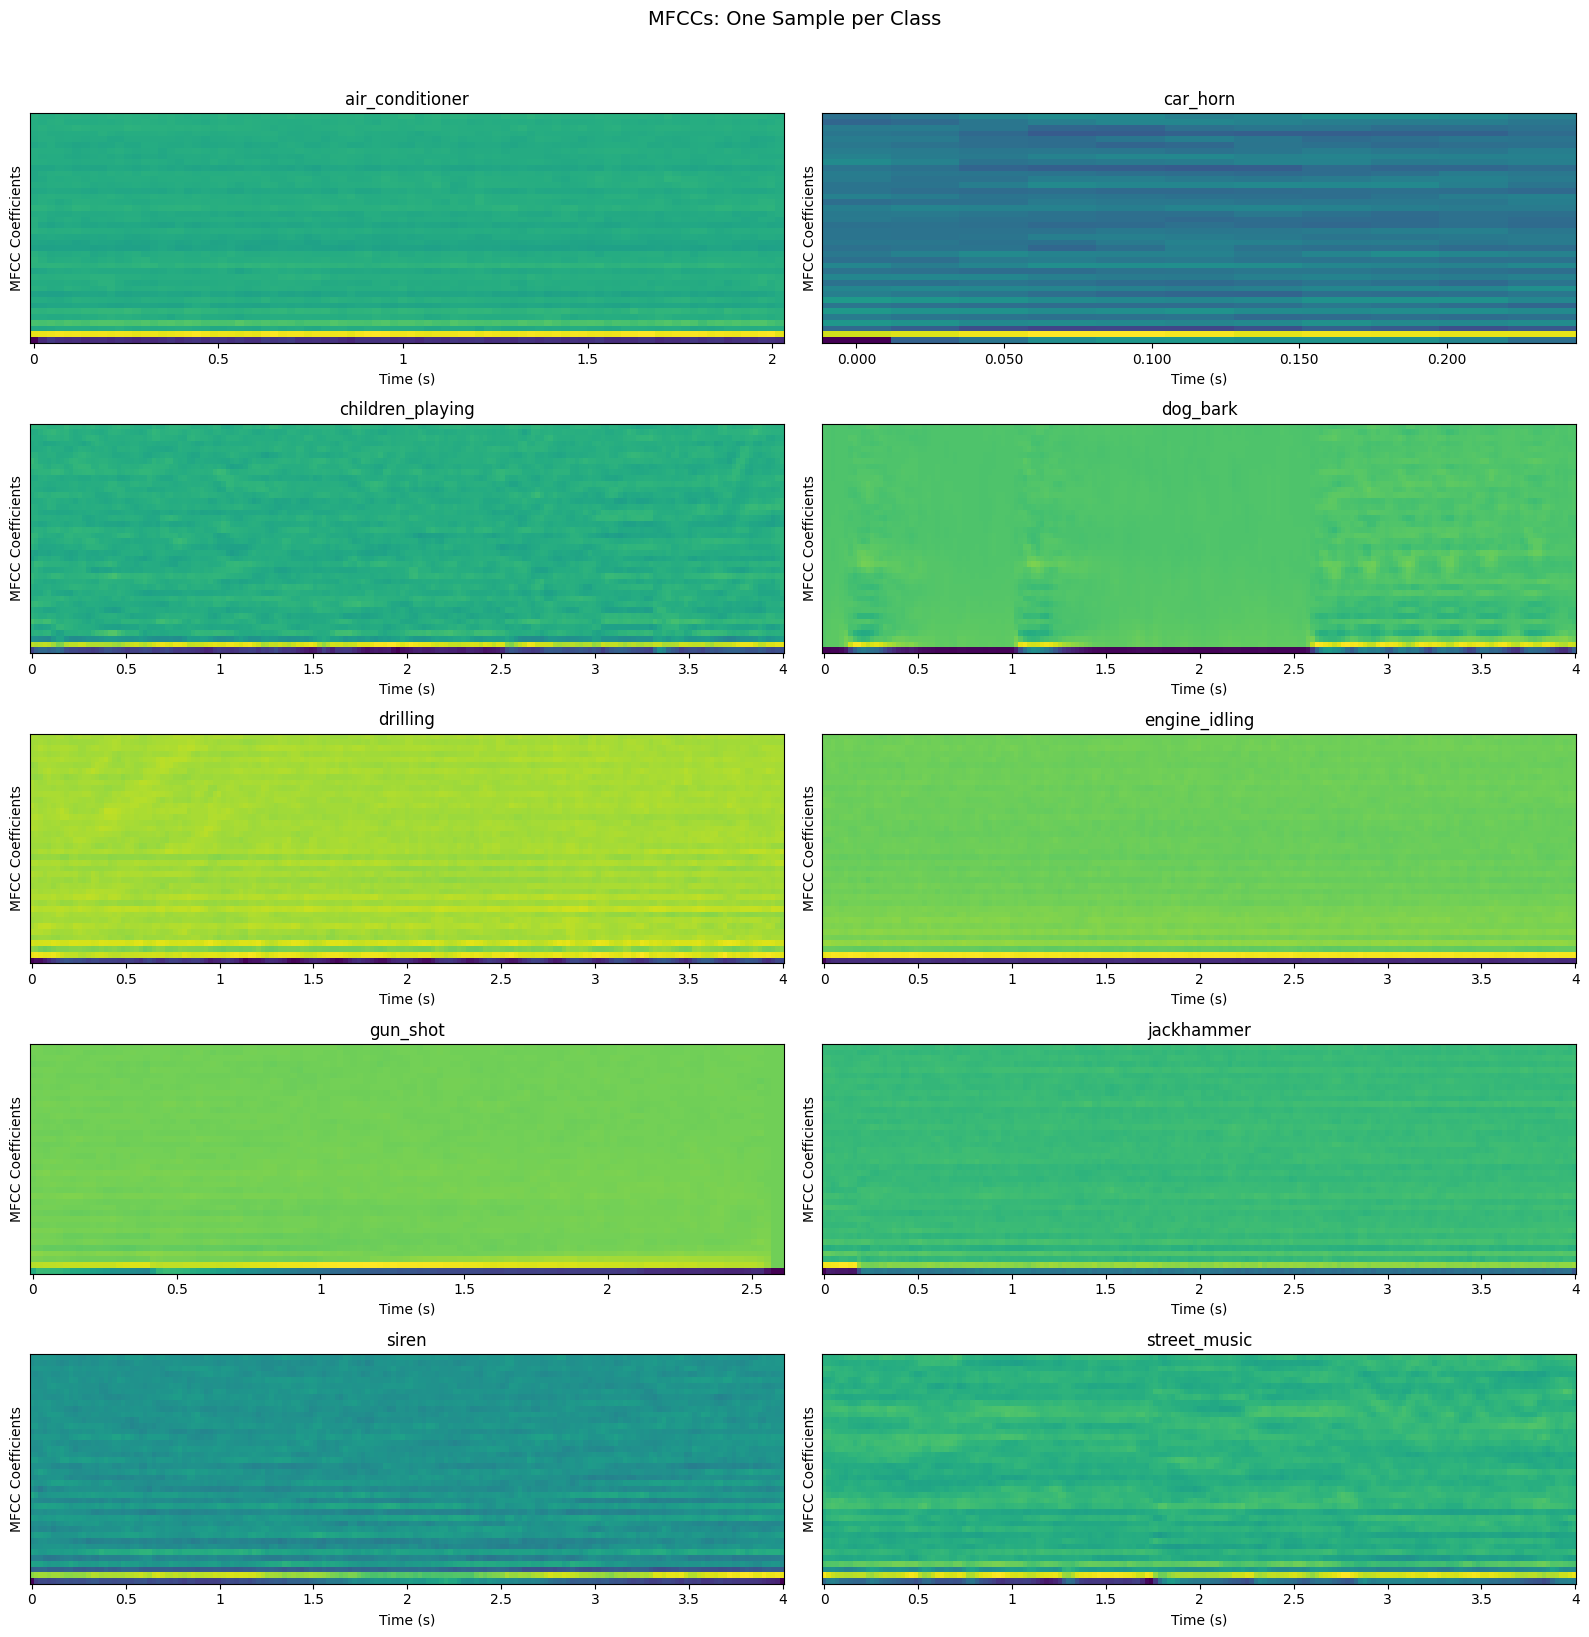
\includegraphics[width=1\linewidth]{Fig/mfcc.png}
    \caption{MFCCs: One Sample per Class}
    \label{fig:mfcc}
\end{figure}

MFCCs are computed by first applying a Short-Time Fourier Transform (STFT) to the audio signal, converting it from the time domain into the frequency domain using overlapping frames. The resulting power spectrum is then mapped onto the Mel scale, a perceptual frequency scale that compresses high-frequency resolution and expands low-frequency resolution, reflecting the non-linear sensitivity of the human ear. Finally, a Discrete Cosine Transform (DCT) is applied to the log-energy Mel filterbank outputs, yielding a compact set of coefficients where the first few capture the most perceptually relevant spectral shape.

For each audio clip in the dataset, 20 MFCC coefficients were extracted per frame using the \textit{librosa} library, with all recordings resampled to 22050 Hz prior to extraction as described in the Data section. These coefficients were then used to create a matrix of shape (20x7), the 7 values representing the min, max, median, mean, kurtosis, variance and skewness of the MFCCs. This makes the representation invariant to temporal alignment and local timing variations, since a very loud sound occuring at frame 10 and one at frame 100 will produce similar statistical profiles if their spectral shape is similar. The seven statistics capture complementary aspects of each coefficient's temporal behavior: the mean and median capture the central tendency of the spectral envelope; the variance and range (min, max) capture how much the spectrum fluctuates over time; and the skewness and kurtosis characterize the shape of the distribution, distinguishing impulsive sounds (high kurtosis, high skewness) from sustained ones (near-Gaussian profiles). The resulting matrices were subsequently flattened into one-dimensional feature vectors of length 140 and standardized using \textit{StandardScaler}, making them serve as the direct input to the clustering algorithms. Class labels were integer-encoded using a label encoder and further converted to a one-hot representation for evaluation purposes, though the clustering step itself operates in an unsupervised manner and does not use label information during training.

\subsection{Determining the Number of Clusters}
\label{section:clusterCount}

Two standard heuristic methods were applied to guide the choice of $k$: the Elbow method and Silhouette analysis.

\subsubsection{Elbow method}

Plots the K-Means inertia (total within-cluster sum of squared distances) as a function of k. The "elbow" suggests a natural cluster count beyond which additional clusters yield diminishing returns.

\subsubsection{Silhouette analysis}

Evaluates partition quality by measuring how well a point fits within its assigned cluster relative to the nearest neighboring cluster:
\[
    s(i) = \frac{b(i) - a(i)}{\max\{a(i),\, b(i)\}}
\]
where $a(i)$ is the mean intra-cluster distance and $b(i)$ is the mean distance to the nearest other cluster. Values close to $+1$ indicate compact, well-separated clusters; values near $0$ indicate boundary points; and negative values indicate likely misassignments.

\subsection{Clustering Algorithms}
\label{section:clusteringAlgorithms}

\subsubsection{K-Means}

K-Means partitions the dataset into $k$ clusters by iteratively assigning each point to its nearest centroid and updating centroids as cluster means. It assumes approximately spherical, equally sized clusters.

\subsubsection{Agglomerative Hierarchical Clustering}

Hierarchical clustering builds a tree of nested partitions by successively merging the two closest clusters. Using Ward's linkage criterion minimizes the increase in total within-cluster variance at each step.

\subsubsection{DBSCAN}

DBSCAN identifies clusters as high-density regions separated by low-density boundaries, without requiring $k$ to be specified in advance. It is controlled by the neighborhood radius ($\varepsilon$) and the minimum number of points required to form a core point. Outliers are explicitly labeled as noise.

\subsection{Visualisation}
\label{section:visualisation}

Since the feature space has 140 dimensions, direct visualisation of cluster assignments is not possible. Two complementary dimensionality reduction techniques were used to project the data into two-dimensional scatter plots for qualitative assessment.

\textbf{PCA} computes a linear projection onto the directions of maximum variance. It provides a faithful, globally structure-preserving view, though it may conceal non-linear separability.

\textbf{t-SNE} applies a non-linear projection that prioritizes preserving local neighborhood relationships, often producing cleaner visual cluster separations.

\subsection{Evaluation Metrics}
Four metrics are computed for each algorithm:
\begin{itemize}
    \item \textbf{Silhouette score} (internal, $\in [-1, 1]$, higher is better): measures the mean ratio of inter-cluster separation to intra-cluster cohesion across all points. A score near $+1$ indicates compact, well-separated clusters; a score near $0$ indicates highly overlapping clusters.

    \item \textbf{Davies--Bouldin index} (internal, $\geq 0$, lower is better): measures the average ratio of within-cluster scatter to between-cluster distance. Lower values indicate better-separated, more compact clusters. An ideal score approaches $0$.

    \item \textbf{Adjusted Rand Index (ARI)} (external, $\in [-1, 1]$, higher is better): measures the agreement between predicted cluster labels and ground-truth class labels, corrected for chance. A score of $0$ indicates random agreement; a score of $1$ indicates a perfect match.

    \item \textbf{Normalised Mutual Information (NMI)} (external, $\in [0, 1]$, higher is better): measures the mutual information between predicted and true labels, normalised to $[0,1]$. Unlike ARI, NMI rewards partial alignment between clusters and classes and is less sensitive to cluster count mismatches.
\end{itemize}

For DBSCAN, internal metrics are computed exclusively on the non-noise subset of the data, as silhouette and Davies--Bouldin scores are undefined for noise points. This introduces a positive bias in DBSCAN's internal metric values relative to K-Means and Hierarchical clustering, and should be taken into account when interpreting the results.


\section{Numerical validation - UrbanSound8K}
\label{section:numericalValidaion}

The experimental evaluation addresses the following central hypothesis: \textit{can unsupervised clustering of MFCC-derived statistical features recover the 10 semantic sound categories of the UrbanSound8K dataset?}

\subsection{Data}

\label{section:data}

The experiments performed in this work are based on the UrbanSound8K dataset. This dataset contains 8732 short audio recordings collected from real urban environments and grouped into 10 semantic sound categories. 

The 10 sound classes available in the dataset are: air\_conditioner, car\_horn, children\_playing, dog\_bark, drilling, engine\_idling, gun\_shot, jackhammer, siren, street\_music.

Before applying clustering algorithms, an exploratory data analysis was performed in order to better understand the structure of the dataset and the acoustic differences between classes.

The first aspect analyzed was the distribution of the sound categories (Figure~\ref{fig:class_distribution}). Although the dataset is relatively balanced, some classes contain fewer examples than others; sounds such as \textit{siren}, \textit{gun\_shot} and \textit{car\_horn} are comparatively underrepresented. This is important because clustering algorithms can be influenced by dominant classes and may produce larger clusters for more frequent sounds.

\begin{figure}[htbp]
    \centering
    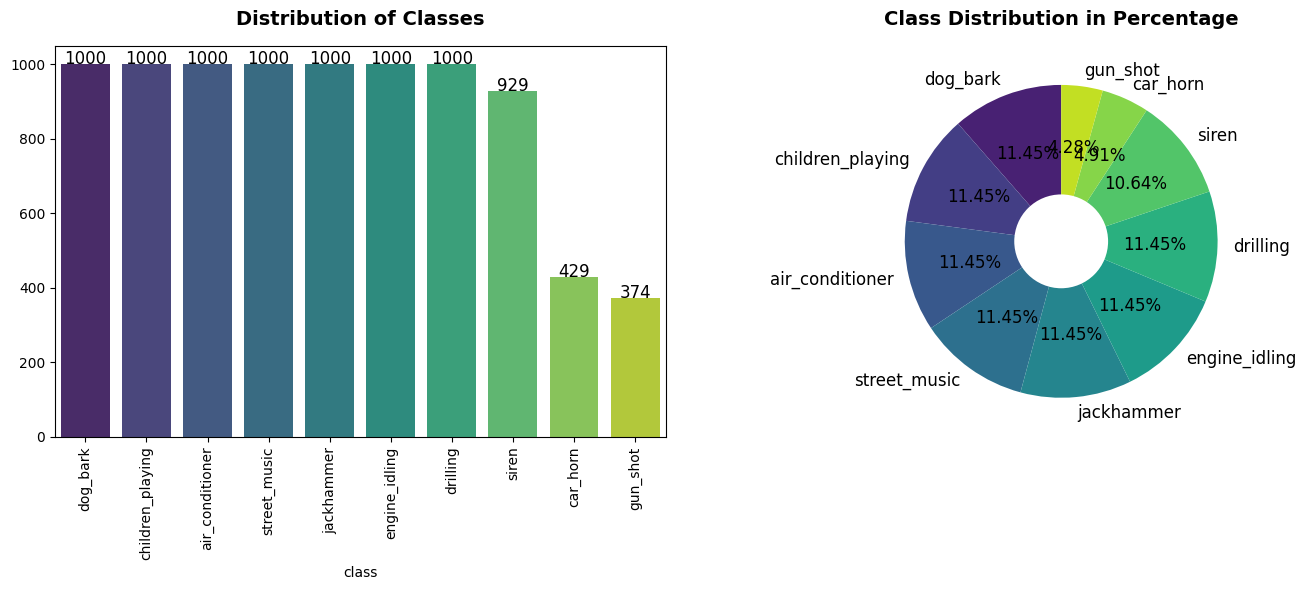
\includegraphics[width=1\linewidth]{Fig/class_distribution.png}
    \caption{UrbanSounds8K Class Distribution}
    \label{fig:class_distribution}
\end{figure}

Another important aspect of the exploratory analysis was the duration of the audio recordings (Figure~\ref{fig:clip_durations}). Most clips have a duration of 4 seconds, but some variability exists across categories. Sounds such as \textit{gun\_shot}, \textit{car\_horn} and \textit{dog\_bark} are usually very short and impulsive, while the others tend to be longer and more continuous.

\begin{figure}[htbp]
    \centering
    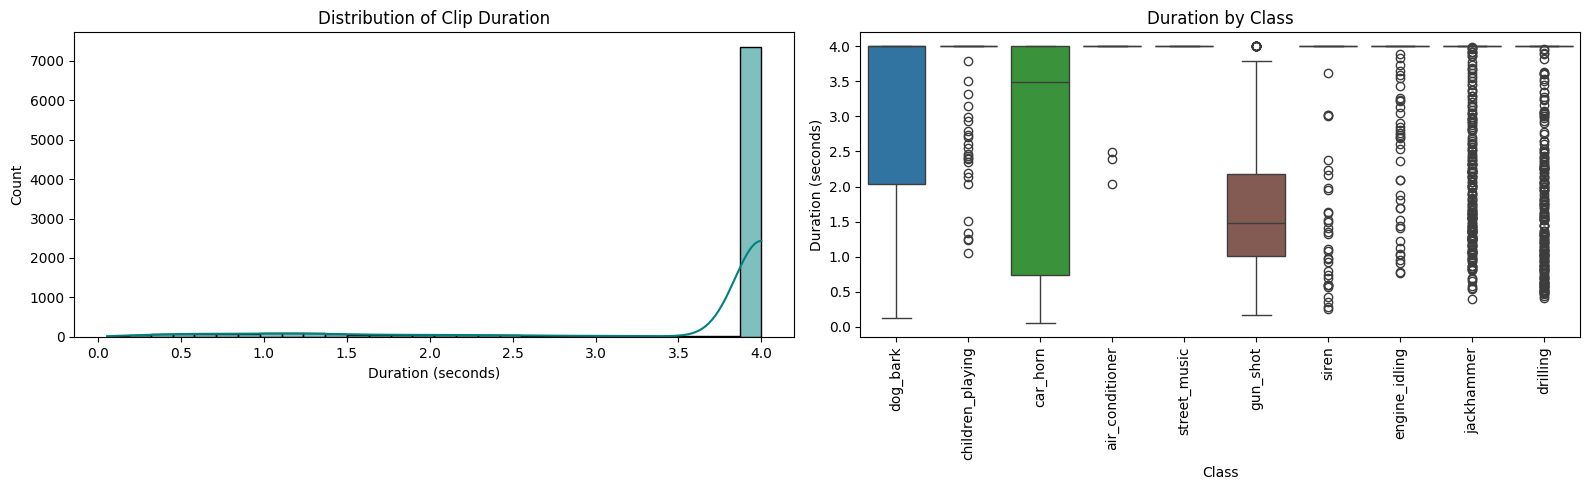
\includegraphics[width=1\linewidth]{Fig/clip_durations.png}
    \caption{Distribuition of Clip Duration}
    \label{fig:clip_durations}
\end{figure}

The sample rate distribution of the UrbanSound8K dataset was also analyzed. Most audio clips are recorded at 44100 Hz, which represents the dominant sample rate in the dataset. The second most common sample rate is 48000 Hz, followed by 96000 Hz. A small number of clips use other sample rates (Figure~\ref{fig:sample_rate_distribution}).

\begin{figure}[htbp]
    \centering
    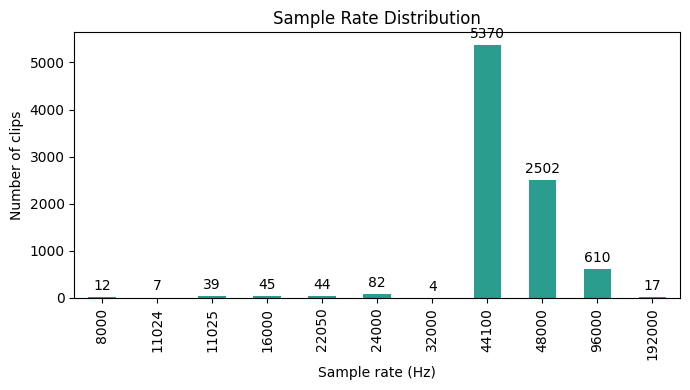
\includegraphics[width=0.5\linewidth]{Fig/sample_rate_distribution.png}
    \caption{Sample Rate Distribution}
    \label{fig:sample_rate_distribution}
\end{figure}

This variability in sample rate can introduce inconsistencies in the extracted audio features, since recordings sampled at different frequencies may contain different amounts of spectral information. In order to ensure that all audio clips have a consistent representation, all recordings are resampled to 22050 Hz before feature extraction.

The choice of 22050 Hz provides a good balance between computational efficiency and sound quality. It is also the default sample rate that the librosa library uses. Resampling all clips to the same frequency also guarantees that the MFCC matrices have comparable dimensions across the entire dataset.

Representative audio clips for each class were also visualized using waveforms. The waveform plots revealed clear differences between sound types. For example, impulsive sounds such as gunshots and dog barks generate sudden peaks in amplitude, while continuous machine sounds such as air conditioners and engine idling produce smoother and more stable waveforms (Figure~\ref{fig:waveforms}).

\begin{figure}[htbp]
    \centering
    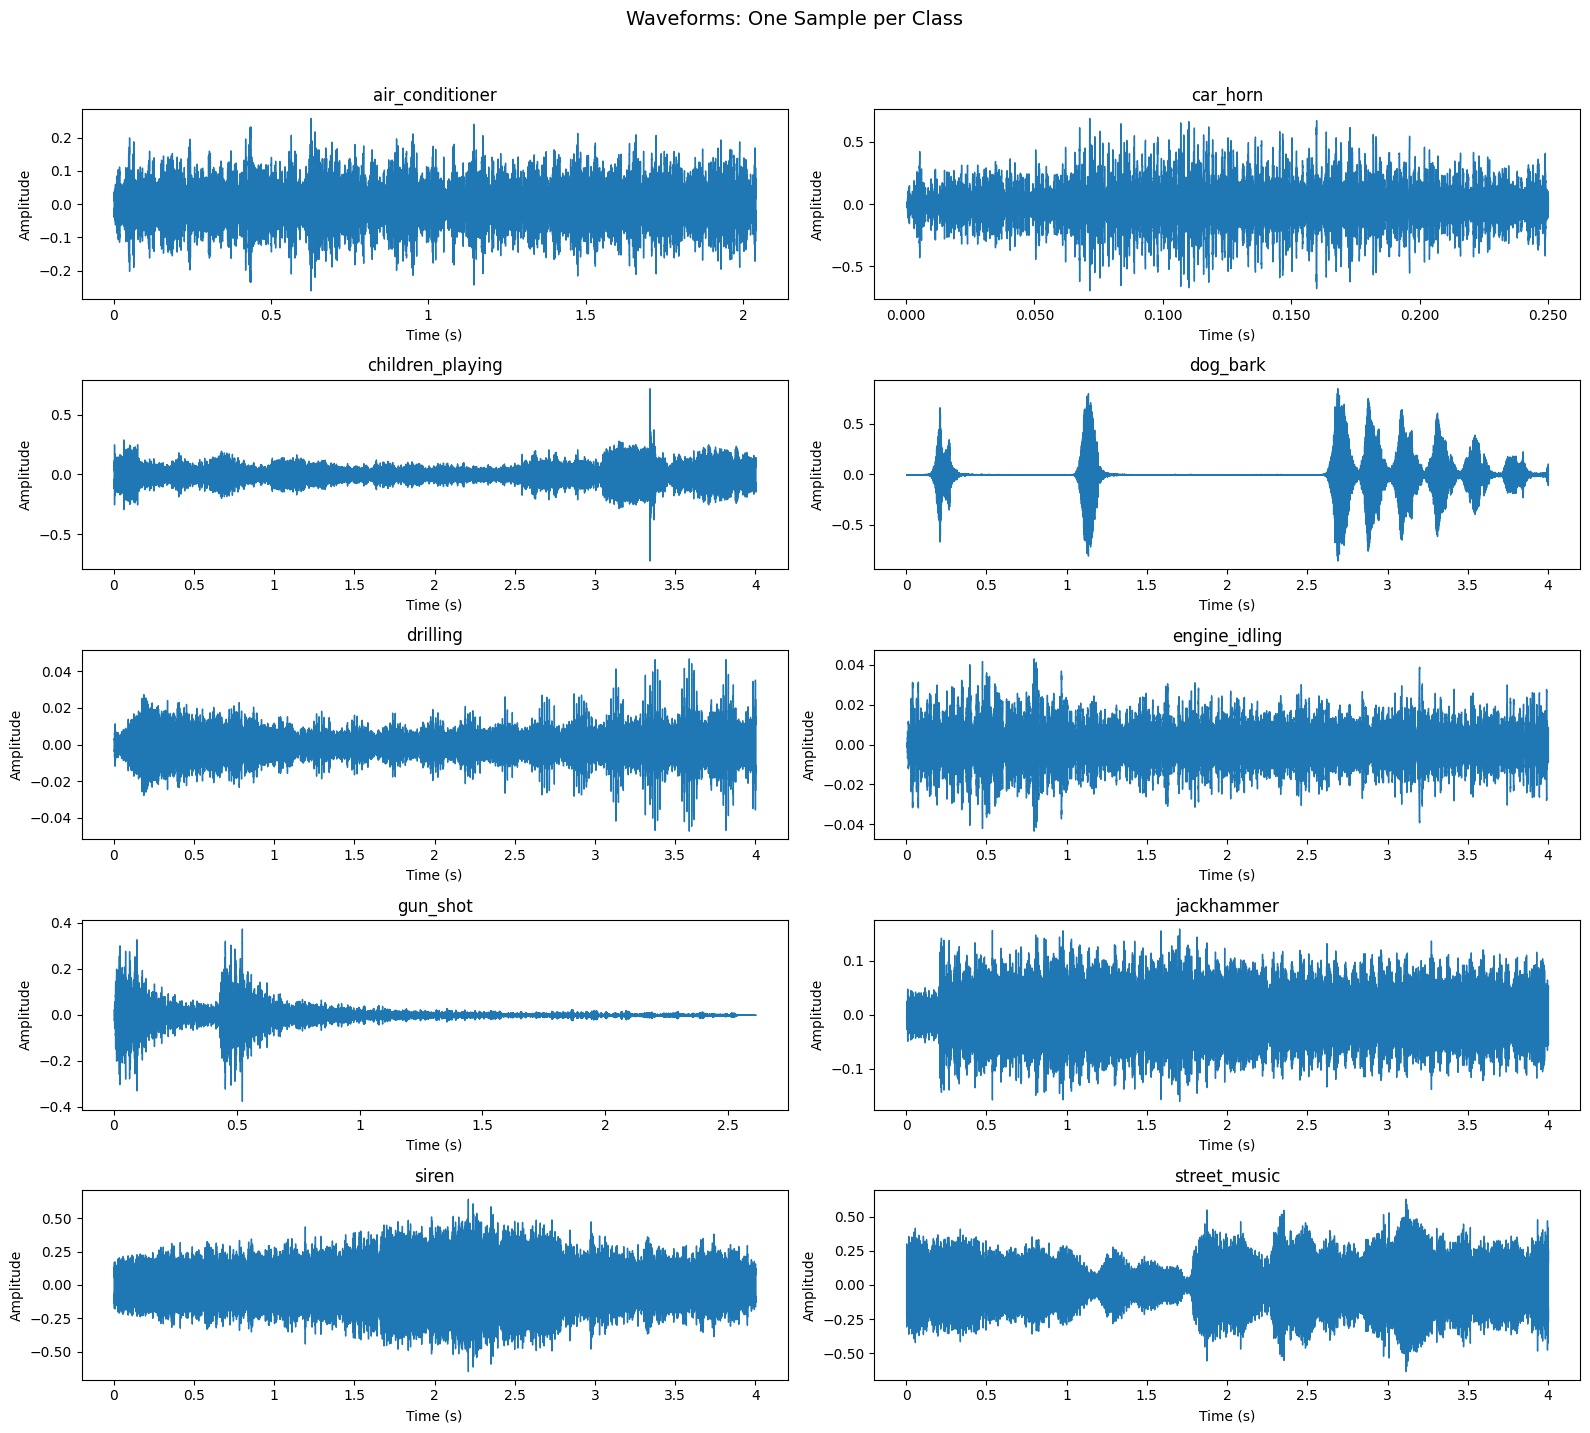
\includegraphics[width=1\linewidth]{Fig/image.png}
    \caption{Waveforms: One Sample per Class}
    \label{fig:waveforms}
\end{figure}

\subsection{Methodology}
\label{section:methodology}

The methodology presented in the previous section was used, with no major changes: the 8,732 audio clips were resampled to 22050 Hz, processed into 140-dimensional statistical MFCC vectors, standardized, and clustered using K-Means, Hierarchical, and DBSCAN. Performance was evaluated using Silhouette, DB, ARI, and NMI.

\subsection{Results}
\label{section:results}

Table~\ref{tab:metrics} summarises the four evaluation metrics for all three algorithms.

\begin{table}[htbp]
    \centering
    \caption{Clustering evaluation metrics. For DBSCAN, internal metrics (Silhouette, Davies--Bouldin) are computed on non-noise points only (21.8\% of the dataset). $\uparrow$ = higher is better; $\downarrow$ = lower is better.}
    \label{tab:metrics}
    \begin{tabular}{lcccc}
        \hline
        \textbf{Algorithm} & \textbf{Silhouette} $\uparrow$ & \textbf{Davies--Bouldin} $\downarrow$ & \textbf{ARI} $\uparrow$ & \textbf{NMI} $\uparrow$ \\
        \hline
        K-Means ($k=10$)       & 0.048  & 2.347  & 0.143  & 0.263  \\
        Hierarchical ($k=10$)  & 0.027  & 2.420  & 0.127  & 0.264  \\
        DBSCAN                 & 0.219* & 1.337* & 0.054* & 0.430* \\
        \hline
        \multicolumn{5}{l}{\small * Computed on non-noise points only.}
    \end{tabular}
\end{table}

\subsubsection{Cluster Structure and Metric Interpretation}

While all three algorithms exhibit relatively low absolute metric values, this reflects a genuine geometric property of the dataset rather than an implementation failure.

K-Means and Hierarchical clustering successfully assigned all 8,732 samples across 10 clusters (100\% coverage). However, their near-zero silhouette scores (0.048 and 0.027, respectively) and high Davies--Bouldin indices indicate poor geometric separation. For both algorithms, the within-cluster spread frequently exceeds the distance to the nearest neighbouring cluster, meaning most points sit close to blurred boundaries rather than firmly within cohesive groups. Despite this, K-Means achieved the highest Adjusted Rand Index (ARI = 0.143), indicating it aligns with the ground-truth semantic classes better than random chance.

Conversely, DBSCAN presents a skewed metric profile. It identified 57 micro-clusters but labelled a staggering 78.2\% of the dataset as noise. While its internal metrics (Silhouette = 0.219, Davies--Bouldin = 1.337) and NMI (0.430) appear superior, these scores are artificially inflated because they are computed exclusively on the densest 21.8\% of the data. The high noise rate confirms that the dataset lacks 10 distinct, compact regions; instead, it occupies a continuous, overlapping volume in the feature space. Consequently, DBSCAN achieved the lowest ARI (0.054) and failed to recover the broad semantic categories.

\subsubsection{Algorithm Comparison}

When evaluating performance, stability, and interpretability for the task of separating the 10 UrbanSound8K categories, the algorithms contrast sharply:

\begin{description}
    \item[Winner: K-Means ($k=10$)] \hfill
    \begin{itemize}
        \item \textbf{Performance:} Achieved the best ground-truth alignment (ARI) with 100\% dataset coverage.
        \item \textbf{Stability:} Highly stable across repeated runs (using k-means++ initialization).
        \item \textbf{Interpretability:} Readily interpretable, as it naturally maps to the 10 target classes and provides distinct cluster centroids representing the ``average'' sound profile of each group.
    \end{itemize}

    \item[Hierarchical Clustering ($k=10$)] \hfill
    \begin{itemize}
        \item \textbf{Drawbacks:} While fully deterministic and producing similar dataset coverage to K-Means, it lacks centroids, making it slightly less interpretable for diagnosing what acoustic profile each cluster represents.
    \end{itemize}

    \item[DBSCAN] \hfill
    \begin{itemize}
        \item \textbf{Drawbacks:} Highly sensitive to hyperparameter tuning ($\varepsilon$ and \texttt{min\_samples}), highly unstable in varying density spaces, and ultimately unsuited for global semantic categorization due to its massive data discard rate.
    \end{itemize}
\end{description}

\subsection{Reasons for Low Overall Performance}

The limited ability of unsupervised clustering to perfectly reconstruct the 10 semantic classes is driven by two overarching constraints:

\begin{enumerate}
    \item \textbf{Data Representation Limits}
    \begin{itemize}
        \item \textbf{Loss of temporal dynamics:} By collapsing the full MFCC matrices into time-averaged statistical summaries (mean, variance, skewness, etc.), the pipeline discarded vital temporal cues like rhythm, onset sharpness, and modulation.
        \item \textbf{Class overlap in MFCC space:} Many classes share near-identical spectral envelopes. For example, continuous mechanical sounds like air conditioner and engine idling are indistinguishable using static moments alone. Without the temporal dimension to separate them, these classes naturally merge into overlapping clusters.
    \end{itemize}

    \item \textbf{Geometric Limits}
    \begin{itemize}
        \item \textbf{Geometric non-separability ($k=2$ vs $k=10$):} The preliminary silhouette sweep suggested $k=2$ as the geometrically optimal partition, naturally separating continuous/tonal sounds from impulsive/transient sounds. Forcing the algorithms to find 10 clusters required them to resolve finer distinctions than the underlying data geometry supported.
        \item \textbf{Curse of dimensionality:} In a 140-dimensional standardized feature space, Euclidean distances between data points converge, eroding the contrast between nearest and farthest neighbours. This inherently weakens distance-based algorithms like K-Means and DBSCAN, resulting in the fuzzy cluster boundaries observed in the visual PCA/t-SNE projections (where the first two principal components explained only 28\% of the total variance).
    \end{itemize}
\end{enumerate}




\subsection{Discussion}
\label{section:discussion}

The experimental results confirm that MFCC-derived statistical features carry partial information about urban sound categories, but are insufficient to drive reliable unsupervised separation of all 10 classes. The hypothesis that clustering can perfectly recover the 10 semantic categories is only weakly supported. In fact, forcing the algorithms to partition the data into 10 distinct groups likely hindered overall performance. While the 10-class approach struggled, a simpler partition of $k = 2$, distinguishing broadly between continuous/sustained sounds and impulsive/transient sounds, remains acoustically viable. This makes sense given the inherent overlap in the feature space: continuous mechanical classes such as \textit{air\_conditioner} and \textit{engine\_idling} sound remarkably similar and share near-identical spectral envelopes. Without richer temporal dynamics, these classes blur together, making artificial separation into 10 groups geometric guesswork rather than genuine acoustic clustering.

The insights gained here regarding algorithm stability, the acoustic overlap of similar classes, and the curse of dimensionality will directly inform the second stage of this work, which focuses on industrial audio data. The clustering pipeline will be ported to the MIMII dataset, shifting the objective from generic sound grouping to practical fault detection. Interestingly, the observation that the pipeline naturally favors a simpler binary partition (like continuous vs. impulsive sounds) aligns perfectly with the end goal of anomaly detection, which seeks to separate normal machine operations from abnormal ones.

While UrbanSound8K presents challenges due to the acoustic overlap of diverse urban categories, industrial audio data from MIMII---containing sounds from specific machines like pumps, valves, fans, and slide rails---may exhibit entirely different clusterability. Unsupervised approaches are highly valuable in these settings because machine faults are often rare, unknown, or difficult to annotate. 

\section{Pipeline Refinements}
\label{section:pipelineRefinements}

The results obtained on the UrbanSound8K dataset revealed two overarching limitations of the baseline pipeline. First, collapsing MFCC trajectories into time-averaged statistical summaries discarded temporal dynamics that are acoustically discriminative: onset sharpness, spectral flux over time, and the rate of change of the spectral envelope were entirely absent from the feature representation. Second, the 140-dimensional feature space exhibited significant inter-class overlap, with many semantically distinct categories sharing nearly identical spectral envelopes when described by static moments alone. The refinements described in this section directly address both of these failure modes, extending the feature representation, replacing the scaler with a more robust alternative, expanding the set of clustering algorithms, and introducing an additional evaluation metric.

\subsection{Feature Augmentation}
\label{section:featureAugmentation}

\subsubsection{Delta MFCCs}

To recover temporal information lost by static MFCC summaries, first-order temporal derivatives of the MFCC coefficients, commonly referred to as delta coefficients, were incorporated into the feature representation. The delta coefficients approximate the rate of change of each MFCC coefficient across adjacent frames, encoding how the spectral envelope evolves over time. This captures acoustically meaningful dynamics such as the sharp onset of an impulsive event or the gradual decay of a sustained tone, which static moment summaries cannot represent. The derivatives were computed using a window width of 3 frames.

The same seven statistical summaries (minimum, maximum, median, mean, variance, skewness, and kurtosis) were applied independently to the delta coefficient trajectories, yielding a second feature matrix of shape $(20 \times 7)$, identical in structure to the original MFCC feature matrix.

\subsubsection{Spectral Contrast}

In addition to cepstral features, spectral contrast was incorporated as a complementary acoustic descriptor. Spectral contrast measures the difference in log energy between spectral peaks and spectral valleys within each of a set of frequency sub-bands. Whereas MFCCs describe the overall shape of the spectral envelope, spectral contrast captures the degree of tonal structure present in a signal: tonal sounds such as sirens and street music tend to exhibit high contrast across sub-bands, while broadband noise sources such as air conditioners and jackhammers tend to exhibit low, uniform contrast. This distinction is largely invisible to MFCC-based representations alone.

Seven sub-bands were used, consistent with the \textit{librosa} default, yielding a coefficient matrix of shape $(7 \times 7)$ after applying the same seven statistical summaries. The resulting 49-dimensional vector was concatenated with the MFCC-derived and delta-derived features, producing a final feature vector of length 329 per audio clip, composed of 140 static MFCC statistics, 140 delta MFCC statistics, and 49 spectral contrast statistics.

\subsubsection{Short Clip Filtering}

During feature extraction, a small subset of clips was found to produce degenerate feature vectors containing \texttt{NaN} or infinite values. This arises from clips that are too short to yield stable MFCC estimates: when too few frames are available, statistical summaries such as variance and kurtosis become unreliable, and edge effects dominate the computed values. Rather than applying an explicit duration threshold, each feature vector was validated numerically after extraction and discarded if any element was non-finite, ensuring that only well-defined representations enter the clustering pipeline.

\subsubsection{Robust Scaling}

The baseline pipeline used z-score normalisation via \textit{StandardScaler}, which standardises each feature dimension to zero mean and unit variance. However, z-score normalisation is sensitive to outliers: extreme values shift the estimated mean and inflate the standard deviation, compressing the bulk of the distribution into a narrow range. Given the heterogeneity of urban audio recordings, which span highly impulsive sounds, sustained tonal signals, and broadband noise, the feature distributions are non-Gaussian and heavy-tailed, making outlier sensitivity a practical concern.

\textit{RobustScaler} was therefore adopted as a replacement. Rather than using the mean and standard deviation, it centres each feature dimension using the median and scales it by the interquartile range (IQR), both of which are resistant to the influence of extreme values. This produces a more stable normalisation across sound classes whose statistical profiles differ markedly in dynamic range.

\subsection{Additional Clustering Methods}
\label{section:additionalClustering}

Two additions were made to the clustering step. The first introduces an entirely new algorithm; the second extends the existing Agglomerative Hierarchical Clustering by evaluating additional linkage criteria.

\subsubsection{Spectral Clustering}

Spectral clustering constructs a $k$-nearest-neighbour similarity graph over the data points and partitions it by embedding the normalised graph Laplacian into a low-dimensional eigenspace, before applying K-Means on the resulting representation. Unlike K-Means operating directly in the original feature space, spectral clustering can recover non-convex cluster shapes and is better suited to datasets where class boundaries are not linearly separable in Euclidean space. The number of clusters $k$ is specified in advance, and a neighbourhood size of 10 nearest neighbours was used to construct the affinity graph.

\subsubsection{Extended Agglomerative Linkage Strategies}

The baseline pipeline applied Agglomerative Hierarchical Clustering exclusively with Ward's linkage criterion, which minimises the increase in total within-cluster variance at each merge step. In the refined pipeline, two additional linkage strategies were evaluated alongside Ward: complete linkage, which merges clusters based on the maximum pairwise distance between their members, and average linkage, which merges based on the mean pairwise distance between all cross-cluster pairs. These alternatives make different geometric assumptions about cluster shape and compactness, and can produce markedly different partitions when clusters are elongated or vary in density. The best-performing linkage strategy was selected based on the Silhouette score, and its results are reported alongside the other algorithms.

\subsection{Extended Evaluation Metrics}
\label{section:extendedMetrics}

The Calinski--Harabasz index was added as a fifth evaluation metric, complementing the four metrics already used in the baseline evaluation.

The \textbf{Calinski--Harabasz index} (internal, $\geq 0$, higher is better) is defined as the ratio of the between-cluster scatter to the within-cluster scatter, both weighted by their respective degrees of freedom:
\[
    \text{CH}(k) = \frac{\mathrm{tr}(B_k)\,/\,(k-1)}{\mathrm{tr}(W_k)\,/\,(n-k)}
\]
where $B_k$ is the between-cluster scatter matrix, $W_k$ is the within-cluster scatter matrix, $k$ is the number of clusters, and $n$ is the total number of samples. Higher values indicate clusters that are simultaneously more compact internally and more separated from one another. The index is undefined for $k = 1$ and tends to favour solutions with a larger number of well-separated clusters, so it is most informative when interpreted alongside the Silhouette score and Davies--Bouldin index rather than in isolation.

\subsection{Dimensionality Reduction as Preprocessing}
\label{section:dimRedPreprocessing}

Given the increase in feature dimensionality from 140 to 329 following feature augmentation, and in light of the curse-of-dimensionality concerns identified in the baseline evaluation, Principal Component Analysis (PCA) was explored as a preprocessing step prior to clustering. The motivation was to reduce noise dimensions and improve the contrast between intra and inter-cluster distances, which tends to erode in high-dimensional Euclidean spaces, while retaining the most variance-bearing directions in the data.

However, clustering on PCA-reduced representations consistently yielded worse scores compared to clustering on the full 329-dimensional feature vectors, regardless of the number of retained components. This outcome suggests that the variance discarded by PCA, despite being quantitatively small in proportion, carries acoustically discriminative information relevant to separating sound classes. The feature space, while high-dimensional, does not appear to be sufficiently redundant to benefit from linear compression prior to clustering, and the cluster separability is not primarily governed by a low-dimensional linear manifold that PCA would expose. Consequently, all clustering experiments reported in the subsequent sections use the full augmented feature vectors without prior dimensionality reduction.

\section{Refined Pipeline Evaluation -- UrbanSound8K}
\label{section:refinedUrbanSound}

The refined pipeline described in Section~\ref{section:pipelineRefinements} was applied to the same UrbanSound8K dataset to assess whether the augmented feature representation, more robust normalisation, and additional clustering algorithms yield measurable improvements over the baseline. Five clips were discarded during feature extraction due to degenerate (non-finite) feature vectors, leaving 8,727 clips for clustering.

\subsection{Results}
\label{section:refinedResults}

Table~\ref{tab:metrics_refined} summarises all five evaluation metrics across four algorithms. The multi-linkage evaluation of Agglomerative Hierarchical Clustering identified \textbf{average linkage} as the best-performing strategy by Silhouette score; this configuration is reported in the table. Figure~\ref{fig:metrics_bar_refined} presents the same values as a grouped bar chart, and Table~\ref{tab:comparison} places the baseline and refined results side by side for K-Means and Hierarchical Clustering.

\begin{table}[htbp]
    \centering
    \small % or \footnotesize
    \caption{Refined pipeline -- clustering evaluation metrics on UrbanSound8K (329-dimensional features, RobustScaler). For DBSCAN, internal metrics are computed on non-noise points only (23.2\% of the dataset). $\uparrow$ = higher is better; $\downarrow$ = lower is better.}
    \label{tab:metrics_refined}
    \begin{tabular}{lccccc}
        \hline
        \textbf{Algorithm} & \textbf{Silhouette} $\uparrow$ & \textbf{Davies--Bouldin} $\downarrow$ & \textbf{Calinski--Harabasz} $\uparrow$ & \textbf{ARI} $\uparrow$ & \textbf{NMI} $\uparrow$ \\
        \hline
        K-Means ($k=10$)                    & 0.147  & 1.849  & 509.2   & 0.075  & 0.223  \\
        Hierarchical (avg linkage)      & 0.807  & 0.511  & 107.0   & 0.000  & 0.006  \\
        DBSCAN                              & 0.071$^*$ & 1.433$^*$ & 32.9$^*$ & $-$0.000$^*$ & 0.154$^*$ \\
        Spectral Clustering ($k=10$)        & $-$0.234 & 1.989 & 90.9   & 0.001  & 0.061  \\
        \hline
        \multicolumn{6}{l}{\footnotesize $^*$ Computed on non-noise points only (76.8\% of clips labelled as noise).}
    \end{tabular}
\end{table}

\begin{table}[htbp]
    \centering
    \caption{Baseline vs.\ refined pipeline -- K-Means. Calinski--Harabasz was not computed in the baseline.}
    \label{tab:comparison}
    \begin{tabular}{llccccc}
        \hline
        \textbf{Pipeline} & \textbf{Algorithm} & \textbf{Silhouette} $\uparrow$ & \textbf{DB} $\downarrow$ & \textbf{CH} $\uparrow$ & \textbf{ARI} $\uparrow$ & \textbf{NMI} $\uparrow$ \\
        \hline
        Baseline & K-Means         & 0.048 & 2.347 & --    & 0.143 & 0.263 \\
        Refined  & K-Means         & 0.147 & 1.849 & 509.2 & 0.075 & 0.223 \\
        \hline
    \end{tabular}
\end{table}

\begin{figure}[htbp]
    \centering
    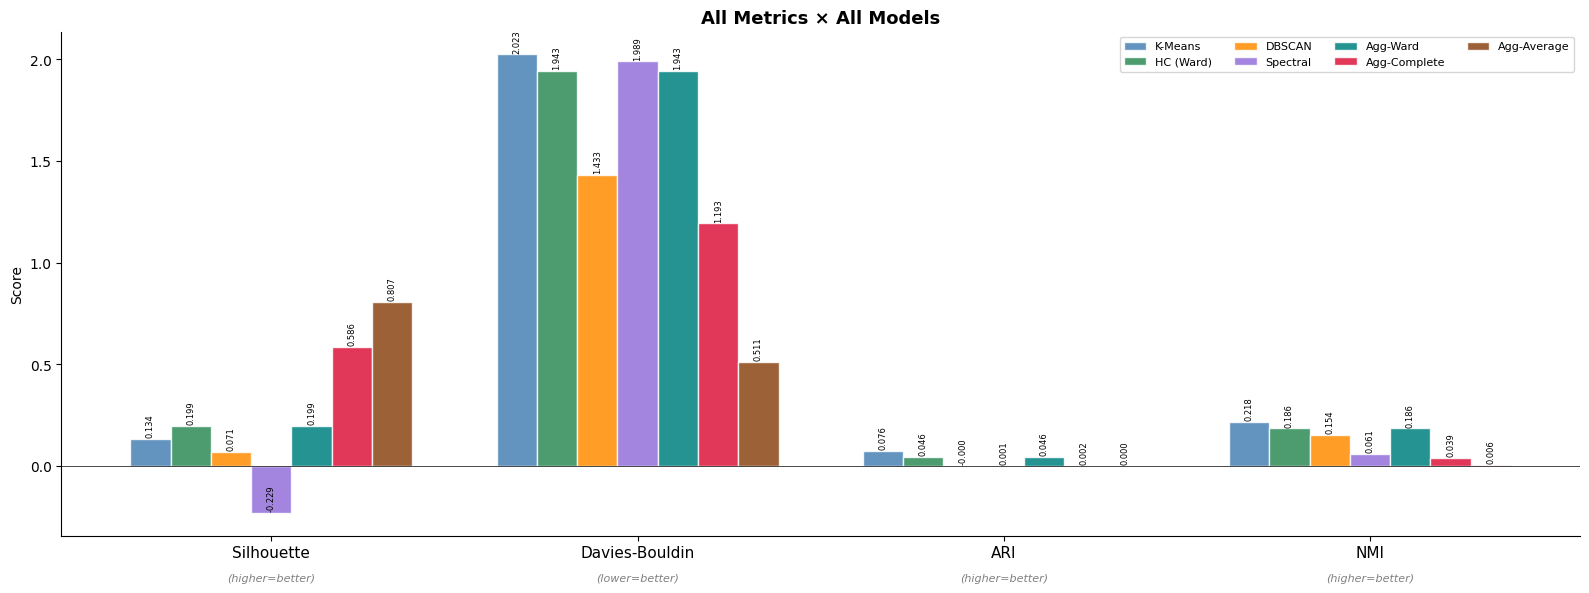
\includegraphics[width=1\linewidth]{Fig/metrics_bar_refined.png}
    \caption{Grouped bar chart of clustering evaluation metrics for the refined pipeline on UrbanSound8K.}
    \label{fig:metrics_bar_refined}
\end{figure}

\subsubsection{K-Means}

K-Means retained 100\% dataset coverage across 10 clusters. Its internal geometry improved substantially relative to the baseline: the Silhouette score rose from 0.048 to 0.147 and the Davies--Bouldin index fell from 2.347 to 1.849, indicating tighter clusters with better inter-cluster separation in the augmented feature space. The Calinski--Harabasz index of 509.2 is the highest among all four algorithms, confirming that K-Means produces the most compact and well-separated partition on this dataset. However, its external metrics declined relative to the baseline: ARI dropped from 0.143 to 0.075, and NMI from 0.263 to 0.223. This divergence suggests that while the 329-dimensional features yield geometrically cleaner clusters, the partition they induce does not align as closely with the ground-truth semantic classes as the 140-dimensional baseline did, pointing to a shift in the structure of the feature space rather than a straightforward improvement.

\subsubsection{Agglomerative Hierarchical Clustering}

The multi-linkage evaluation revealed a striking stratification across the three strategies. Average linkage achieved the highest Silhouette score (0.807) and the lowest Davies--Bouldin index (0.511) by a large margin, while complete linkage obtained intermediate values (Silhouette = 0.570, DB = 1.193), and Ward linkage -- the only strategy used in the baseline -- produced the weakest internal scores (Silhouette = 0.198, DB = 1.943). These large differences in internal metrics are, however, accompanied by near-zero ARI and NMI values for both average (ARI = 0.000, NMI = 0.006) and complete linkage (ARI = 0.002, NMI = 0.039). This pattern is characteristic of degenerate partitions: average and complete linkage collapse almost all points into one or two giant clusters and scatter the remainder into tiny singleton-like groups, achieving an artificially smooth internal geometry at the cost of any meaningful semantic structure. Ward linkage, despite its lower Silhouette score (0.198), produces a far more balanced partition (ARI = 0.046, NMI = 0.186) and remains the practically superior choice when external alignment with ground-truth classes is the objective.

\subsubsection{Spectral Clustering}

Spectral Clustering produced the weakest results across virtually all metrics: a negative Silhouette score ($-$0.234), the highest Davies--Bouldin index (1.989), and near-zero ARI (0.001) and NMI (0.061). The negative Silhouette score indicates that, on average, points are closer to a neighbouring cluster than to their own assigned cluster -- meaning the graph-based affinity partitioning failed to recover cohesive groups in the 329-dimensional space. This may reflect the difficulty of constructing a meaningful $k$-nearest-neighbour graph in a high-dimensional space where distance contrasts are inherently weakened by the curse of dimensionality.

\subsubsection{DBSCAN}

DBSCAN labelled 76.8\% of the dataset (6,704 clips) as noise and identified only 14 micro-clusters. Its internal metrics computed on the retained 23.2\% subset (Silhouette = 0.071, DB = 1.433, CH = 32.9) are inflated by selection bias and should not be compared directly to the full-coverage algorithms. Its ARI of effectively zero ($-$0.000) confirms that it recovers no meaningful semantic structure. The noise rate is nearly identical to the baseline result (78.2\%), confirming that the augmented feature representation does not resolve the fundamental lack of compact density regions that DBSCAN requires.

\subsubsection{Algorithm Comparison}

When evaluating performance for the task of recovering the 10 UrbanSound8K semantic categories, the algorithms contrast as follows in the refined pipeline:

\begin{description}
    \item[Winner: K-Means ($k=10$)] \hfill
    \begin{itemize}
        \item \textbf{Performance:} Best ARI (0.075) and NMI (0.223) among all algorithms, with 100\% dataset coverage. Highest Calinski--Harabasz index (509.2), confirming the strongest ratio of between-cluster to within-cluster scatter.
        \item \textbf{Geometry vs.\ semantics:} Internal metrics improved substantially over the baseline (Silhouette $+$0.099, DB $-$0.498), but external metrics declined (ARI $-$0.068, NMI $-$0.040), revealing that the augmented feature space reshapes cluster geometry without necessarily aligning that geometry more closely with semantic class boundaries.
    \end{itemize}

    \item[Hierarchical Clustering -- Ward linkage] \hfill
    \begin{itemize}
        \item \textbf{Practical choice:} Although average linkage dominates on internal metrics, Ward linkage is the only agglomerative strategy that produces a balanced partition with meaningful external alignment (ARI = 0.046, NMI = 0.186). The multi-linkage sweep thus confirms Ward as the appropriate default for this task.
        \item \textbf{Drawbacks:} External metrics remain below K-Means, and the algorithm lacks centroids, limiting interpretability.
    \end{itemize}

    \item[Spectral Clustering ($k=10$)] \hfill
    \begin{itemize}
        \item \textbf{Drawbacks:} The negative Silhouette score and near-zero external metrics indicate that graph-based affinity partitioning is poorly suited to this high-dimensional, overlapping feature space. Its additional computational cost (affinity graph construction and eigendecomposition) is not justified by the results.
    \end{itemize}

    \item[DBSCAN] \hfill
    \begin{itemize}
        \item \textbf{Drawbacks:} Massive noise rate (76.8\%), effectively zero ARI, and metric values computed on a heavily biased subset render it unsuited for global semantic categorisation regardless of the feature representation used.
    \end{itemize}
\end{description}

\subsection{Discussion}
\label{section:refinedDiscussion}

The refined pipeline yields a more nuanced picture than a straightforward improvement over the baseline. The augmented 329-dimensional feature representation demonstrably improves the internal geometry of K-Means clusters: tighter within-cluster cohesion and greater inter-cluster separation are reflected in the higher Silhouette and lower Davies--Bouldin scores. Yet the external metrics -- ARI and NMI -- both declined, meaning the new clusters are geometrically cleaner but semantically less aligned with the ground-truth class labels. This dissociation reveals that the additional features introduced by delta coefficients and spectral contrast reshape the feature space in ways that do not necessarily amplify the dimensions that discriminate between semantic categories. The richer representation captures more acoustic variance, but not all of that variance is semantically informative.

The multi-linkage agglomerative experiment underscores a broader risk: optimising for internal metrics alone can be deeply misleading. Average linkage achieves a Silhouette score of 0.807 -- far above any other configuration -- but its ARI of 0.000 exposes this as a degenerate outcome where nearly all data collapses into one cluster. This serves as a concrete cautionary example for why internal and external metrics must be interpreted together, and why the Calinski--Harabasz index, while useful, must similarly be examined alongside ground-truth-based measures.

Spectral Clustering's poor performance across all metrics reinforces the curse-of-dimensionality concern identified in the baseline analysis. In a 329-dimensional space where Euclidean distances converge, the $k$-nearest-neighbour graph no longer provides meaningful local structure, and the graph Laplacian eigenvectors fail to reveal separable clusters. PCA preprocessing was explored precisely to mitigate this, but -- as noted in Section~\ref{section:dimRedPreprocessing} -- it consistently worsened results, confirming that no low-dimensional linear manifold captures the relevant structure.

The silhouette sweep again identified $k = 2$ as the geometrically optimal partition, consistent with the baseline finding. This persistent preference for a binary separation of impulsive and sustained sounds, even after substantial feature augmentation, reinforces the conclusion that the pipeline is naturally better suited to coarser distinctions than to fine-grained 10-class recovery. This observation directly motivates the transition to the MIMII dataset, where the objective is precisely such a binary partition: separating normal machine operation from anomalous behaviour.

\section{Numerical Validation - MIMII}
\label{section:numericalValidationMIMII}

Having validated the refined clustering pipeline on UrbanSound8K, the same methodology was applied to the MIMII dataset to address the central motivating question of this work: \textit{can the unsupervised clustering pipeline distinguish normal industrial machine operation from anomalous behaviour without access to fault labels during training?} Unlike the 10-class semantic recovery task posed by UrbanSound8K, MIMII frames clustering as a binary partitioning problem, the kind of coarse, two-way separation that the silhouette sweeps in both baseline and refined pipelines consistently identified as the most geometrically natural outcome for this feature representation.

\subsection{Data}
\label{section:dataMIMII}

The MIMII (Malfunctioning Industrial Machine Investigation and Inspection) dataset was used to evaluate the pipeline in an industrial fault-detection setting. The portion of the dataset used in this work contains 2,279 audio recordings collected from four types of industrial machines: \textit{fan}, \textit{pump}, \textit{slider} (slide rail), and \textit{valve}. Each clip is labelled with a binary condition, \textit{normal} or \textit{abnormal}, derived directly from the folder structure of the dataset (machine type / condition / clip), so no separate metadata file is required. The dataset contains no missing values and no duplicate file paths.

\begin{figure}[htbp]
    \centering
    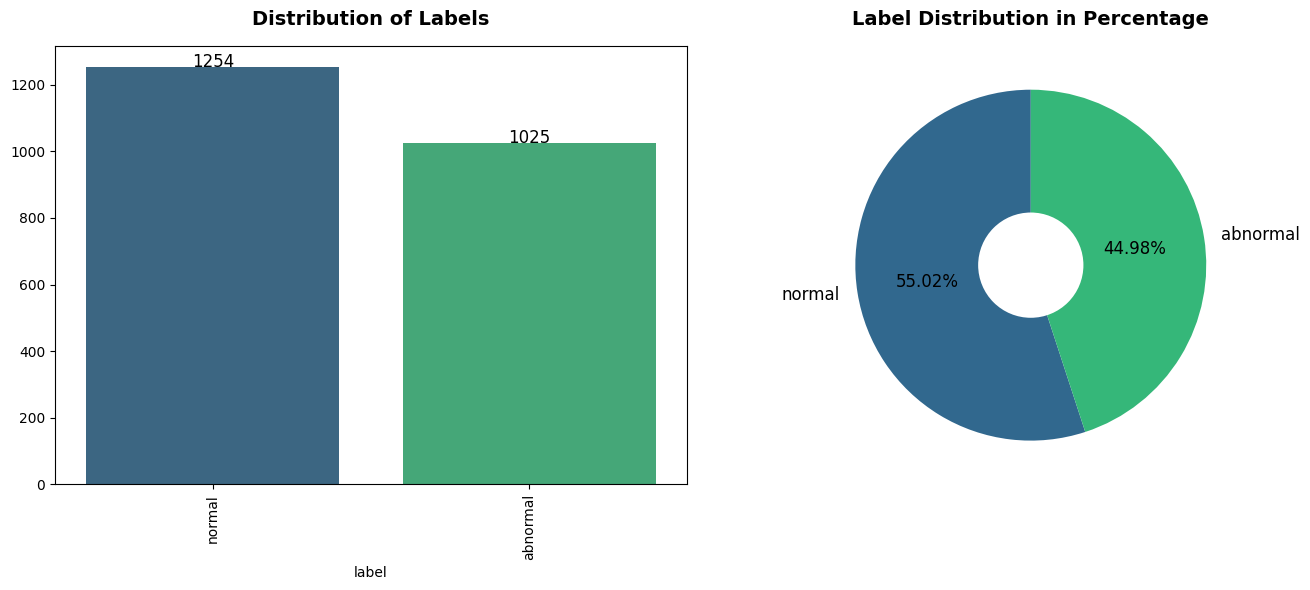
\includegraphics[width=\linewidth]{Fig/mimii_class_distribution.png}
    \caption{Distribution of labels across the MIMII dataset. Normal clips (1{,}254) slightly outnumber abnormal clips (1{,}025), yielding a near-balanced split of 55\% vs.\ 45\%.}
    \label{fig:mimii_class_dist}
\end{figure}

\begin{figure}[htbp]
    \centering
    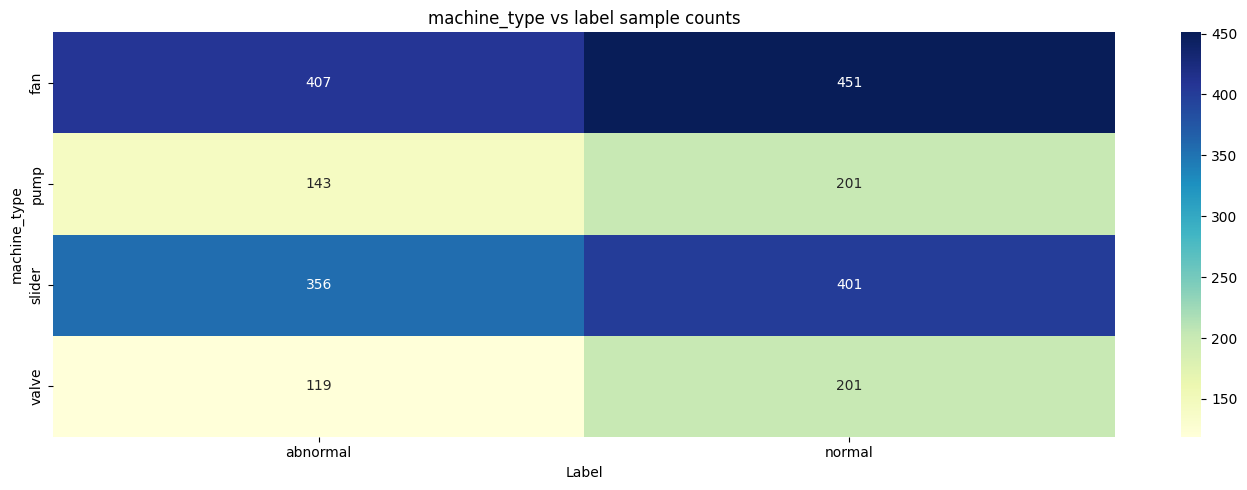
\includegraphics[width=\linewidth]{Fig/mimii_counts.png}
    \caption{Sample counts per machine type and label.}
    \label{fig:mimii_counts}
\end{figure}

Unlike UrbanSound8K, where sample rates varied substantially across clips, all MIMII recordings are sampled uniformly at 16{,}000\,Hz (Figure~\ref{fig:mimii_sr}). This eliminates one source of inter-clip variability and removes the need for resampling: the feature extractor was configured with \texttt{sr=16000} to operate on the audio at its native rate. Clip durations are likewise homogeneous, with all recordings of similar length (Figure~\ref{fig:mimii_durations}), which contrasts with the duration heterogeneity observed in UrbanSound8K.

\begin{figure}[htbp]
    \centering
    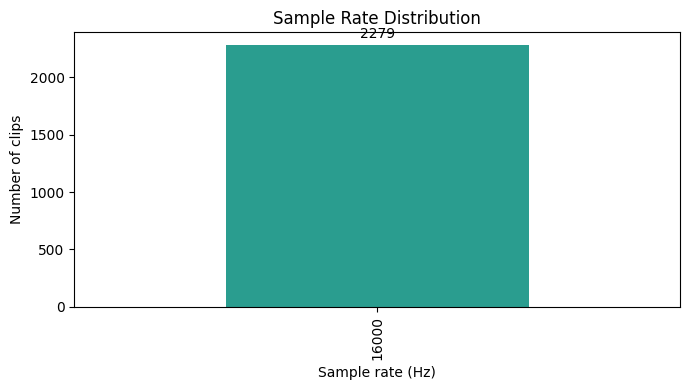
\includegraphics[width=0.6\linewidth]{Fig/mimii_sr.png}
    \caption{Sample rate distribution. All 2,279 clips are recorded at 16{,}000\,Hz, requiring no resampling.}
    \label{fig:mimii_sr}
\end{figure}

\begin{figure}[htbp]
    \centering
    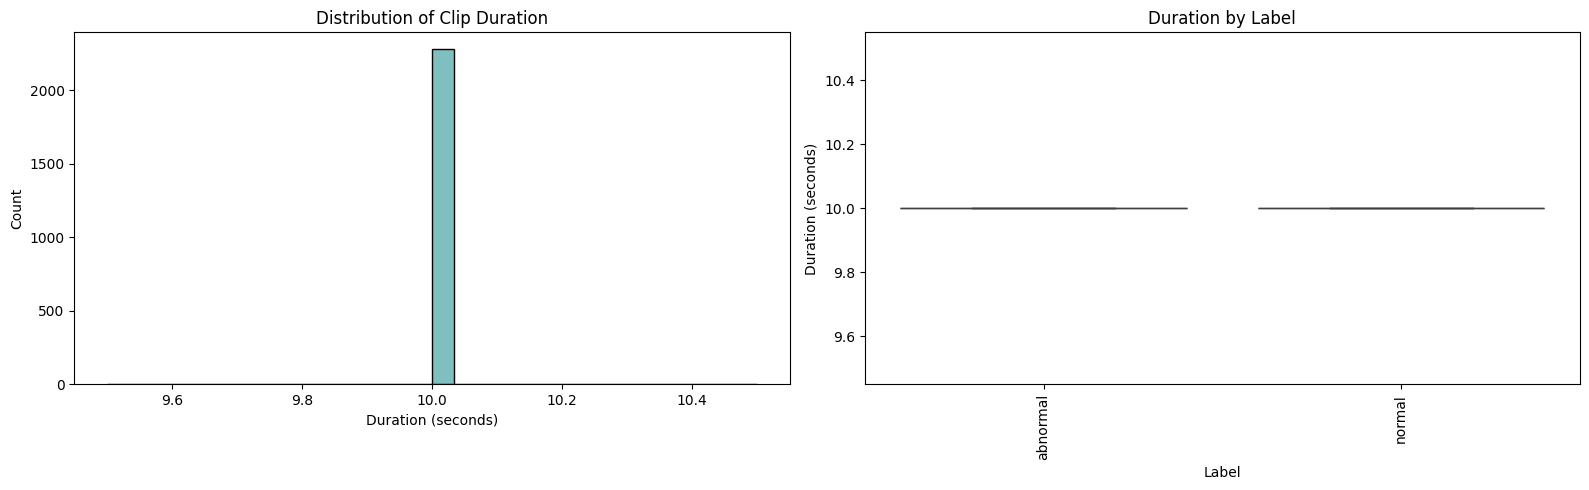
\includegraphics[width=\linewidth]{Fig/mimii_clip_durations.png}
    \caption{Clip duration distribution. All recordings are uniformly 10 seconds long, with no variance between normal and abnormal classes.}
    \label{fig:mimii_durations}
\end{figure}

\subsection{Methodology}
\label{section:methodologyMIMII}

The refined pipeline described in Section~\ref{section:pipelineRefinements} was applied without structural modification. The only change relative to the UrbanSound8K configuration was the audio loading sample rate, set to 16000 Hz to match MIMII's native sampling. All other steps remained identical: 20 MFCC coefficients per frame, first-order delta MFCCs computed with a window width of 3 frames, and spectral contrast over seven sub-bands; the same seven statistical summaries (minimum, maximum, median, mean, variance, skewness, and kurtosis) applied to each coefficient trajectory; concatenation into a 329-dimensional feature vector per clip; numerical validation to discard any non-finite vectors; and \textit{RobustScaler} normalisation. No clips were discarded during extraction. The final feature matrix has shape $(2279 \times 329)$.

The same six clustering configurations evaluated on UrbanSound8K were applied to MIMII: K-Means, Hierarchical Clustering with Ward linkage, DBSCAN, Spectral Clustering, and Agglomerative Clustering with complete and average linkage. The number of clusters was set to $k = 2$ to match the binary ground-truth labelling (normal versus abnormal). The DBSCAN $\varepsilon$ parameter was selected automatically from the 15th percentile of the $k$-distance distribution, as before, yielding $\varepsilon = 10.54$ with \texttt{min\_samples} $= 10$. All five evaluation metrics (Silhouette, Davies--Bouldin, Calinski--Harabasz, ARI, NMI) were computed, with DBSCAN's internal metrics again restricted to the non-noise subset of the data. PCA and t-SNE projections were generated for visual inspection; PCA's first two components explained 29.5\% of the total variance, comparable to UrbanSound8K (28\%).

\subsection{Results}
\label{section:resultsMIMII}

Table~\ref{tab:metrics_mimii} summarises the five evaluation metrics across all configurations. The K-Means silhouette sweep over $k \in [2, 19]$ identified $k = 3$ as the geometrically optimal partition by silhouette score, with $k = 2$ (the ground-truth condition labelling) as the second-best choice. The reported clustering results all use $k = 2$ to align directly with the binary normal/abnormal target.

\begin{table}[htbp]
    \centering
    \small
    \caption{Refined pipeline -- clustering evaluation metrics on MIMII (329-dimensional features, RobustScaler, $k=2$). For DBSCAN, internal metrics are computed on non-noise points only (25.5\% of the dataset). $\uparrow$ = higher is better; $\downarrow$ = lower is better.}
    \label{tab:metrics_mimii}
    \begin{tabular}{lccccc}
        \hline
        \textbf{Algorithm} & \textbf{Silhouette} $\uparrow$ & \textbf{Davies--Bouldin} $\downarrow$ & \textbf{Calinski--Harabasz} $\uparrow$ & \textbf{ARI} $\uparrow$ & \textbf{NMI} $\uparrow$ \\
        \hline
        K-Means ($k=2$)                     & 0.189   & 2.336   & 394.3   & 0.060   & 0.041   \\
        Hierarchical (Ward)                 & 0.219   & 2.286   & 366.1   & 0.000   & 0.009   \\
        Agglomerative (complete)            & 0.369   & 0.932   & 32.7    & 0.002   & 0.010   \\
        Agglomerative (average)             & 0.488   & 0.387   & 6.2     & 0.000   & 0.001   \\
        Spectral Clustering ($k=2$)         & 0.227   & 2.010   & 273.9   & $-$0.005 & 0.004  \\
        DBSCAN                              & 0.176$^*$ & 1.825$^*$ & 77.1$^*$ & $-$0.070$^*$ & 0.113$^*$ \\
        \hline
        \multicolumn{6}{l}{\footnotesize $^*$ Computed on non-noise points only (74.5\% of clips labelled as noise).}
    \end{tabular}
\end{table}

\subsubsection{K-Means}

K-Means with $k = 2$ retained 100\% dataset coverage and produced the highest external metric values among all configurations evaluated, with ARI = 0.060 and NMI = 0.041. Internally, it achieved a Silhouette score of 0.189, a Davies--Bouldin index of 2.336, and the highest Calinski--Harabasz index of all algorithms at 394.3, indicating the strongest overall ratio of between-cluster to within-cluster scatter when both clusters retain a substantial fraction of the data. Despite leading the external metrics, the absolute values remain extremely low: an ARI of 0.060 represents only a marginal improvement over chance agreement with the binary condition labels, indicating that the two clusters K-Means produces do not meaningfully separate normal from abnormal clips.

\subsubsection{Agglomerative Hierarchical Clustering}

The multi-linkage evaluation reveals the same pattern observed on UrbanSound8K, but more starkly. Ward linkage produced a balanced two-cluster partition (Silhouette = 0.219, Davies--Bouldin = 2.286) with effectively zero external alignment (ARI = 0.000, NMI = 0.009). Complete linkage achieved a substantially higher Silhouette score (0.369) and a much lower Davies--Bouldin index (0.932) but again with negligible external scores (ARI = 0.002, NMI = 0.010). Average linkage maximised the internal geometry (Silhouette = 0.488, Davies--Bouldin = 0.387) while collapsing into a near-degenerate partition with ARI = 0.000 and NMI = 0.001. The pattern is identical to the UrbanSound8K observation: the linkage strategies with the cleanest internal geometry achieve that geometry by funnelling almost all of the data into one cluster and leaving a small residue in the other, an outcome that maximises silhouette by construction but carries no semantic content.

\subsubsection{Spectral Clustering}

Spectral Clustering with $k = 2$ produced a Silhouette score of 0.227, the second-highest among the balanced (non-degenerate) configurations, and a Davies--Bouldin index of 2.010, marginally better than K-Means and Ward hierarchical. However, its external metrics are essentially indistinguishable from random assignment, with ARI = $-$0.005 and NMI = 0.004. The negative ARI confirms that the graph-based partition is uncorrelated with the normal/abnormal labelling. Compared to its catastrophic performance on UrbanSound8K (Silhouette $= -0.234$), Spectral Clustering recovers a coherent geometric partition on MIMII; the binary task is geometrically easier than the 10-class one. The partition simply does not align with the supervised label of interest.

\subsubsection{DBSCAN}

DBSCAN's behaviour on MIMII differs qualitatively from every other algorithm. It labelled 74.5\% of the dataset (1,697 clips) as noise and identified two clusters in the remaining 25.5\% (582 clips). On this non-noise subset, it produced a Silhouette score of 0.176, a Davies--Bouldin index of 1.825, and a Calinski--Harabasz index of 77.1.

Two aspects of the DBSCAN result are notable. First, its ARI is negative ($-0.070$), the lowest of any algorithm, indicating that its retained clusters are systematically anti-correlated with the normal/abnormal labelling on the non-noise subset. Second, despite this, it achieves the highest NMI among all algorithms (0.113), more than twice the value of any other method. The combination of negative ARI and positive NMI is informative: NMI rewards any structured relationship between the predicted partition and the true labels, regardless of direction, while ARI penalises misalignment. The fact that DBSCAN carries more mutual information about the labels than any other algorithm, but in a direction that disagrees with the intended normal/abnormal axis, suggests that its dense regions correspond to a different latent structure in the data, almost certainly machine type rather than condition. Normal clips of a single machine type form acoustically tight, homogeneous regions in the feature space; abnormal clips, being statistical deviations from those baselines, are pushed to the periphery and flagged as noise. The 74.5\% noise rate is consistent with this reading: it approximately matches the share of the dataset that lies outside the densest machine-type-specific normal-operation regions.

\subsubsection{Algorithm Comparison}

When evaluating performance for the task of separating normal from abnormal MIMII clips, the algorithms contrast as follows:

\begin{description}
    \item[Winner on external metrics: K-Means ($k=2$)] \hfill
    \begin{itemize}
        \item \textbf{Performance:} Highest ARI (0.060) and NMI (0.041) among full-coverage algorithms, but absolute values remain very low. Highest Calinski--Harabasz index (394.3) among all algorithms.
        \item \textbf{Limitation:} The partition that K-Means recovers is only marginally correlated with the normal/abnormal label. It produces the best of a uniformly weak set of results.
    \end{itemize}

    \item[Best internal geometry: Agglomerative (average linkage)] \hfill
    \begin{itemize}
        \item \textbf{Performance:} Highest Silhouette (0.488) and lowest Davies--Bouldin (0.387) of all algorithms, but this reflects a degenerate partition with one giant cluster and one tiny one (ARI = 0.000).
        \item \textbf{Lesson:} As on UrbanSound8K, optimising for internal metrics alone selects a meaningless solution.
    \end{itemize}

    \item[Most label-informative geometry: DBSCAN] \hfill
    \begin{itemize}
        \item \textbf{Performance:} Highest NMI (0.113), but negative ARI ($-0.070$). The retained 25.5\% of the data carries more information about labels than any other algorithm's output, but the information appears to encode machine type rather than condition.
        \item \textbf{Drawback:} 74.5\% of the data is discarded, making DBSCAN unsuitable as a global classifier even if its dense regions are semantically meaningful for a different purpose.
    \end{itemize}

    \item[Spectral Clustering and Hierarchical (Ward)] \hfill
    \begin{itemize}
        \item \textbf{Drawbacks:} Both produce balanced two-cluster partitions with reasonable internal geometry (Silhouette $\approx 0.22$) but no external alignment with the normal/abnormal labels (ARI $\leq 0.001$).
    \end{itemize}
\end{description}

\subsection{Discussion}
\label{section:discussionMIMII}

The MIMII results lead to a more pessimistic but more informative conclusion than the UrbanSound8K results. The pipeline does succeed in finding geometrically coherent two-cluster partitions of the data, the silhouette and Davies--Bouldin scores attained by K-Means, Hierarchical (Ward), and Spectral Clustering are comparable to or better than what was achieved on UrbanSound8K at $k = 10$, but the partitions it finds are not aligned with the normal/abnormal axis that the task requires. All ARI values lie within $[-0.07, 0.06]$, a band that is statistically indistinguishable from chance for a balanced two-class problem.

The most plausible explanation, and the one most consistent with the DBSCAN evidence, is that the dominant source of variation in the 329-dimensional feature space is machine type, not condition. A fan, a pump, a slide rail, and a valve produce acoustically very different signals: their spectral envelopes, their delta-MFCC profiles, and their spectral contrast distributions occupy clearly separated regions of the feature space. The difference between a normal fan and an abnormal fan, by contrast, is small relative to the difference between any fan and any valve. When clustering is asked to find two groups in this space, the geometry it discovers is shaped by the machine-type axis: the two clusters K-Means produces are not normal-versus-abnormal but rather some grouping of machines against others. The corroborating evidence from DBSCAN, where ARI is negative against the normal/abnormal label but NMI is the highest of any algorithm, is consistent with this reading. DBSCAN finds dense, homogeneous regions in the feature space, and those regions correspond to normal-operation clips of individual machine types, with abnormal clips falling outside as noise.

This finding has direct implications for the use of unsupervised clustering as a fault-detection method on MIMII. Naively clustering the full dataset into two groups does not produce a normal-versus-abnormal partition. The latent machine-type structure dominates and must be controlled for before clustering can recover the condition axis. Two natural remedies follow from this analysis: clustering each machine type independently, so that the only remaining axis of variation within each sub-population is condition; or applying anomaly-detection methods that explicitly model a per-machine "normal" baseline (such as one-class support vector machines, isolation forests, or autoencoder reconstruction error) rather than treating the problem as symmetric two-class clustering. Both approaches would respect the structural property of the dataset that has emerged from the present analysis: that ``normal'' and ``abnormal'' are not two acoustic categories on equal footing, but rather a baseline-and-deviation pair defined relative to a specific machine.

A secondary observation reinforces a methodological point already made in the UrbanSound8K analysis: internal metrics, when used in isolation, can be actively misleading. Average linkage achieves the highest Silhouette score on MIMII (0.488) and the lowest Davies--Bouldin index (0.387), values that on their face suggest an exceptionally clean partition. The accompanying ARI of 0.000 reveals this as a degenerate outcome. The Calinski--Harabasz index, newly introduced in the refined pipeline, is informative here precisely because it penalises this degeneracy: average linkage's Calinski--Harabasz of 6.2 is the lowest of any algorithm, correctly flagging that the partition has very little between-cluster scatter relative to its within-cluster scatter once the imbalance is accounted for. This confirms the recommendation, already made in Section~\ref{section:refinedDiscussion}, that internal metrics be interpreted jointly across multiple indices and always alongside external metrics where any form of ground truth is available.

Finally, the silhouette sweep again identified a number of clusters one greater than the ground-truth count ($k = 3$ versus the true $k = 2$) as geometrically optimal, mirroring the persistent tendency observed on UrbanSound8K for the pipeline to prefer a slightly coarser or different partition than the supervised labelling suggests. This is consistent with the interpretation above: the feature space's natural decomposition reflects the machine-type / dominant-mode structure of the data rather than the binary condition label, and the silhouette-optimal $k$ is sensitive to that intrinsic structure rather than to the external task definition.

In summary, the refined clustering pipeline transfers cleanly from UrbanSound8K to MIMII as a software artefact, but the binary fault-detection task on the full MIMII dataset proves to be ill-posed under symmetric clustering: the dominant geometric structure of the feature space encodes machine identity rather than operational condition, and recovering the condition axis from these features will require either per-machine treatment or an asymmetric, baseline-relative formulation of the anomaly-detection problem.





\chapter{Conclusion and future work}
\label{chapter:concl}

This report asked whether unsupervised clustering of acoustic features can group sounds meaningfully without manual labels -- first as a proof of concept on urban audio, then as a fault-detection tool on industrial machine sound. A single modular pipeline was applied unchanged to both datasets, yielding one positive engineering result and one informative negative result that together show where unsupervised clustering helps and where it does not.

\section{Summary of findings}
\label{section:summaryFindings}

On UrbanSound8K, MFCC statistical features carried only partial information about the ten categories. K-Means gave the best alignment with the ground-truth labels (ARI = 0.143), but agreement was modest, and every silhouette sweep favoured a coarse two-way split between sustained and impulsive sounds. Adding temporal derivatives and spectral contrast improved cluster geometry (Silhouette 0.048~$\rightarrow$~0.147, Davies--Bouldin 2.347~$\rightarrow$~1.849) but reduced semantic alignment (ARI 0.143~$\rightarrow$~0.075) -- geometric cleanliness and semantic correctness are distinct goals. This was reinforced by the hierarchical experiment, where average linkage scored a near-perfect Silhouette of 0.807 while collapsing almost all clips into one cluster (ARI = 0.000): internal metrics alone can be misleading.

On the industrial MIMII dataset, no algorithm separated normal from abnormal operation -- every ARI fell within $\pm0.07$ of chance. DBSCAN was diagnostic: its clusters were the most label-informative (highest NMI = 0.113) yet \emph{negatively} aligned with the normal/abnormal label (ARI = $-0.070$). The dominant axis of variation encodes \emph{machine type}, not operating condition; a normal and an abnormal fan are more alike than either is to a valve, so symmetric two-way clustering recovers machine identity rather than machine health.

\section{SWOT analysis}
\label{section:swot}

\begin{description}
    \item[Strengths] \hfill
    \begin{itemize}
        \item A modular pipeline that transferred from urban to industrial audio.
        \item Rigorous evaluation combining internal and external metrics.
        \item Fully unsupervised, matching settings where fault labels are rare.
        \item Interpretable, theory-grounded features and algorithms.
        \item A machine-type-versus-condition finding that usefully redirects future effort.
    \end{itemize}

    \item[Weaknesses] \hfill
    \begin{itemize}
        \item Time-averaged statistics discard temporal dynamics. \emph{Remedy:} sequence models or spectrogram embeddings.
        \item Distance-based clustering degrades in 329 dimensions. \emph{Remedy:} compact learned representations.
        \item Symmetric framing mismatches an asymmetric problem. \emph{Remedy:} anomaly detection or per-machine clustering.
        \item Heuristic hyperparameters. \emph{Remedy:} systematic model selection.
        \item Narrow evaluation. \emph{Remedy:} more machine types and benchmarks.
    \end{itemize}

    \item[Opportunities] \hfill
    \begin{itemize}
        \item Self-supervised audio representations for more discriminative features.
        \item Per-machine anomaly detection for real-time predictive maintenance.
        \item Feature disentanglement to remove device and environment confounds.
        \item Semi-supervised use of the few fault labels that exist.
    \end{itemize}

    \item[Threats] \hfill
    \begin{itemize}
        \item Domain shift across factories, microphones, and noise profiles.
        \item Rare faults complicating thresholds and evaluation.
        \item Concept drift as machines age.
        \item High cost of false alarms and missed detections in safety contexts.
    \end{itemize}
\end{description}

\section{Ethical considerations and business impact}
\label{section:ethics}

Both datasets embed biases that propagate into the clusters: their categories and ``normal'' baselines reflect the machines, conditions, and recording devices that were sampled, and the microphone and signal chain can cause clusters to track device artefacts rather than acoustic content -- exactly the machine-identity confound observed on MIMII. MIMII's near-balanced 55\%/45\% split is also unrepresentative of reality, where faults are rare, so balanced evaluation flatters the task. Privacy is a first-order concern: always-on workplace microphones are a potential surveillance apparatus, so any deployment should process audio on-device, retain only derived features, and obtain worker consent.

The approach is relatively interpretable, which is an ethical asset for safety-relevant decisions, and a per-machine, baseline-relative formulation is fairer than global clustering because it judges each machine against its own normal behaviour. The costs of errors are asymmetric: a missed fault is dangerous, while repeated false alarms erode trust and cause alarm fatigue. Because this pipeline does not reliably separate normal from abnormal on the full MIMII dataset, it should be presented as a decision-support tool that augments human judgement, never an autonomous safety guarantee, with accountability resting on the humans and processes around it. Commercially, cheap retrofittable microphones make acoustic monitoring attractive for predictive maintenance, but this specific pipeline is a well-characterised research artefact rather than a production-ready product.

\section{Future work and outlook}
\label{section:futureWork}

The clearest direction is to abandon the symmetric two-way framing for a per-machine, baseline-relative one: model each machine's normal operation and flag deviations, via per-machine clustering or dedicated anomaly detection. The second priority is representation learning -- a compact, temporally aware embedding (autoencoders or self-supervised models) would address both the curse of dimensionality and the loss of temporal information. The main contribution of this work is therefore not a winning algorithm but a clear account of when acoustic clustering works and why it fails: internal metrics must never be read in isolation, and naive clustering of mixed-machine audio recovers \emph{equipment identity}, not \emph{equipment health}. That insight steers future work away from a tempting but ill-posed approach and toward the formulation that can actually work.








\bibliographystyle{plain}
\bibliography{BibAll}

\end{document}

